% Created by tikzDevice version 0.12.3.1 on 2023-06-22 09:01:49
% !TEX encoding = UTF-8 Unicode
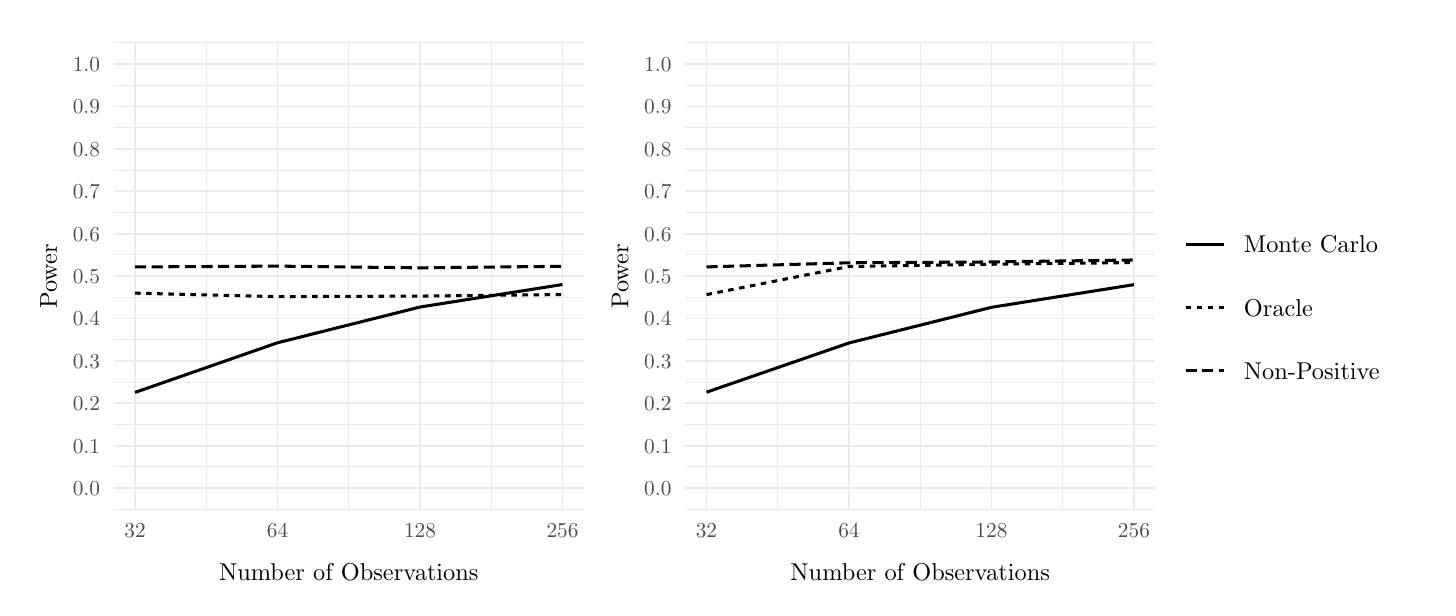
\begin{tikzpicture}[x=1pt,y=1pt]
\definecolor{fillColor}{RGB}{255,255,255}
\path[use as bounding box,fill=fillColor,fill opacity=0.00] (0,0) rectangle (505.89,202.36);
\begin{scope}
\path[clip] ( 31.08, 28.32) rectangle (200.99,196.86);
\definecolor{drawColor}{gray}{0.92}

\path[draw=drawColor,line width= 0.3pt,line join=round] ( 31.08, 28.32) --
	(200.99, 28.32);

\path[draw=drawColor,line width= 0.3pt,line join=round] ( 31.08, 43.64) --
	(200.99, 43.64);

\path[draw=drawColor,line width= 0.3pt,line join=round] ( 31.08, 58.96) --
	(200.99, 58.96);

\path[draw=drawColor,line width= 0.3pt,line join=round] ( 31.08, 74.28) --
	(200.99, 74.28);

\path[draw=drawColor,line width= 0.3pt,line join=round] ( 31.08, 89.60) --
	(200.99, 89.60);

\path[draw=drawColor,line width= 0.3pt,line join=round] ( 31.08,104.93) --
	(200.99,104.93);

\path[draw=drawColor,line width= 0.3pt,line join=round] ( 31.08,120.25) --
	(200.99,120.25);

\path[draw=drawColor,line width= 0.3pt,line join=round] ( 31.08,135.57) --
	(200.99,135.57);

\path[draw=drawColor,line width= 0.3pt,line join=round] ( 31.08,150.89) --
	(200.99,150.89);

\path[draw=drawColor,line width= 0.3pt,line join=round] ( 31.08,166.21) --
	(200.99,166.21);

\path[draw=drawColor,line width= 0.3pt,line join=round] ( 31.08,181.53) --
	(200.99,181.53);

\path[draw=drawColor,line width= 0.3pt,line join=round] ( 31.08,196.86) --
	(200.99,196.86);

\path[draw=drawColor,line width= 0.3pt,line join=round] ( 64.55, 28.32) --
	( 64.55,196.86);

\path[draw=drawColor,line width= 0.3pt,line join=round] (116.04, 28.32) --
	(116.04,196.86);

\path[draw=drawColor,line width= 0.3pt,line join=round] (167.52, 28.32) --
	(167.52,196.86);

\path[draw=drawColor,line width= 0.6pt,line join=round] ( 31.08, 35.98) --
	(200.99, 35.98);

\path[draw=drawColor,line width= 0.6pt,line join=round] ( 31.08, 51.30) --
	(200.99, 51.30);

\path[draw=drawColor,line width= 0.6pt,line join=round] ( 31.08, 66.62) --
	(200.99, 66.62);

\path[draw=drawColor,line width= 0.6pt,line join=round] ( 31.08, 81.94) --
	(200.99, 81.94);

\path[draw=drawColor,line width= 0.6pt,line join=round] ( 31.08, 97.27) --
	(200.99, 97.27);

\path[draw=drawColor,line width= 0.6pt,line join=round] ( 31.08,112.59) --
	(200.99,112.59);

\path[draw=drawColor,line width= 0.6pt,line join=round] ( 31.08,127.91) --
	(200.99,127.91);

\path[draw=drawColor,line width= 0.6pt,line join=round] ( 31.08,143.23) --
	(200.99,143.23);

\path[draw=drawColor,line width= 0.6pt,line join=round] ( 31.08,158.55) --
	(200.99,158.55);

\path[draw=drawColor,line width= 0.6pt,line join=round] ( 31.08,173.87) --
	(200.99,173.87);

\path[draw=drawColor,line width= 0.6pt,line join=round] ( 31.08,189.20) --
	(200.99,189.20);

\path[draw=drawColor,line width= 0.6pt,line join=round] ( 38.81, 28.32) --
	( 38.81,196.86);

\path[draw=drawColor,line width= 0.6pt,line join=round] ( 90.29, 28.32) --
	( 90.29,196.86);

\path[draw=drawColor,line width= 0.6pt,line join=round] (141.78, 28.32) --
	(141.78,196.86);

\path[draw=drawColor,line width= 0.6pt,line join=round] (193.26, 28.32) --
	(193.26,196.86);
\definecolor{drawColor}{RGB}{0,0,0}

\path[draw=drawColor,line width= 1.1pt,line join=round] ( 38.81, 70.56) --
	( 90.29, 88.50) --
	(141.78,101.41) --
	(193.26,109.55);

\path[draw=drawColor,line width= 1.1pt,dash pattern=on 2pt off 2pt ,line join=round] ( 38.81,106.43) --
	( 90.29,105.16) --
	(141.78,105.37) --
	(193.26,105.92);

\path[draw=drawColor,line width= 1.1pt,dash pattern=on 4pt off 2pt ,line join=round] ( 38.81,115.90) --
	( 90.29,116.20) --
	(141.78,115.57) --
	(193.26,116.14);
\end{scope}
\begin{scope}
\path[clip] (  0.00,  0.00) rectangle (505.89,202.36);
\definecolor{drawColor}{gray}{0.30}

\node[text=drawColor,anchor=base east,inner sep=0pt, outer sep=0pt, scale=  0.77] at ( 26.13, 33.33) {0.0};

\node[text=drawColor,anchor=base east,inner sep=0pt, outer sep=0pt, scale=  0.77] at ( 26.13, 48.65) {0.1};

\node[text=drawColor,anchor=base east,inner sep=0pt, outer sep=0pt, scale=  0.77] at ( 26.13, 63.97) {0.2};

\node[text=drawColor,anchor=base east,inner sep=0pt, outer sep=0pt, scale=  0.77] at ( 26.13, 79.29) {0.3};

\node[text=drawColor,anchor=base east,inner sep=0pt, outer sep=0pt, scale=  0.77] at ( 26.13, 94.61) {0.4};

\node[text=drawColor,anchor=base east,inner sep=0pt, outer sep=0pt, scale=  0.77] at ( 26.13,109.94) {0.5};

\node[text=drawColor,anchor=base east,inner sep=0pt, outer sep=0pt, scale=  0.77] at ( 26.13,125.26) {0.6};

\node[text=drawColor,anchor=base east,inner sep=0pt, outer sep=0pt, scale=  0.77] at ( 26.13,140.58) {0.7};

\node[text=drawColor,anchor=base east,inner sep=0pt, outer sep=0pt, scale=  0.77] at ( 26.13,155.90) {0.8};

\node[text=drawColor,anchor=base east,inner sep=0pt, outer sep=0pt, scale=  0.77] at ( 26.13,171.22) {0.9};

\node[text=drawColor,anchor=base east,inner sep=0pt, outer sep=0pt, scale=  0.77] at ( 26.13,186.54) {1.0};
\end{scope}
\begin{scope}
\path[clip] (  0.00,  0.00) rectangle (505.89,202.36);
\definecolor{drawColor}{gray}{0.30}

\node[text=drawColor,anchor=base,inner sep=0pt, outer sep=0pt, scale=  0.77] at ( 38.81, 18.06) {32};

\node[text=drawColor,anchor=base,inner sep=0pt, outer sep=0pt, scale=  0.77] at ( 90.29, 18.06) {64};

\node[text=drawColor,anchor=base,inner sep=0pt, outer sep=0pt, scale=  0.77] at (141.78, 18.06) {128};

\node[text=drawColor,anchor=base,inner sep=0pt, outer sep=0pt, scale=  0.77] at (193.26, 18.06) {256};
\end{scope}
\begin{scope}
\path[clip] (  0.00,  0.00) rectangle (505.89,202.36);
\definecolor{drawColor}{RGB}{0,0,0}

\node[text=drawColor,anchor=base,inner sep=0pt, outer sep=0pt, scale=  0.88] at (116.04,  2.52) {Number of Observations};
\end{scope}
\begin{scope}
\path[clip] (  0.00,  0.00) rectangle (505.89,202.36);
\definecolor{drawColor}{RGB}{0,0,0}

\node[text=drawColor,rotate= 90.00,anchor=base,inner sep=0pt, outer sep=0pt, scale=  0.88] at ( 10.57,112.59) {Power};
\end{scope}
\begin{scope}
\path[clip] (237.57, 28.32) rectangle (407.47,196.86);
\definecolor{drawColor}{gray}{0.92}

\path[draw=drawColor,line width= 0.3pt,line join=round] (237.57, 28.32) --
	(407.47, 28.32);

\path[draw=drawColor,line width= 0.3pt,line join=round] (237.57, 43.64) --
	(407.47, 43.64);

\path[draw=drawColor,line width= 0.3pt,line join=round] (237.57, 58.96) --
	(407.47, 58.96);

\path[draw=drawColor,line width= 0.3pt,line join=round] (237.57, 74.28) --
	(407.47, 74.28);

\path[draw=drawColor,line width= 0.3pt,line join=round] (237.57, 89.60) --
	(407.47, 89.60);

\path[draw=drawColor,line width= 0.3pt,line join=round] (237.57,104.93) --
	(407.47,104.93);

\path[draw=drawColor,line width= 0.3pt,line join=round] (237.57,120.25) --
	(407.47,120.25);

\path[draw=drawColor,line width= 0.3pt,line join=round] (237.57,135.57) --
	(407.47,135.57);

\path[draw=drawColor,line width= 0.3pt,line join=round] (237.57,150.89) --
	(407.47,150.89);

\path[draw=drawColor,line width= 0.3pt,line join=round] (237.57,166.21) --
	(407.47,166.21);

\path[draw=drawColor,line width= 0.3pt,line join=round] (237.57,181.53) --
	(407.47,181.53);

\path[draw=drawColor,line width= 0.3pt,line join=round] (237.57,196.86) --
	(407.47,196.86);

\path[draw=drawColor,line width= 0.3pt,line join=round] (271.04, 28.32) --
	(271.04,196.86);

\path[draw=drawColor,line width= 0.3pt,line join=round] (322.52, 28.32) --
	(322.52,196.86);

\path[draw=drawColor,line width= 0.3pt,line join=round] (374.01, 28.32) --
	(374.01,196.86);

\path[draw=drawColor,line width= 0.6pt,line join=round] (237.57, 35.98) --
	(407.47, 35.98);

\path[draw=drawColor,line width= 0.6pt,line join=round] (237.57, 51.30) --
	(407.47, 51.30);

\path[draw=drawColor,line width= 0.6pt,line join=round] (237.57, 66.62) --
	(407.47, 66.62);

\path[draw=drawColor,line width= 0.6pt,line join=round] (237.57, 81.94) --
	(407.47, 81.94);

\path[draw=drawColor,line width= 0.6pt,line join=round] (237.57, 97.27) --
	(407.47, 97.27);

\path[draw=drawColor,line width= 0.6pt,line join=round] (237.57,112.59) --
	(407.47,112.59);

\path[draw=drawColor,line width= 0.6pt,line join=round] (237.57,127.91) --
	(407.47,127.91);

\path[draw=drawColor,line width= 0.6pt,line join=round] (237.57,143.23) --
	(407.47,143.23);

\path[draw=drawColor,line width= 0.6pt,line join=round] (237.57,158.55) --
	(407.47,158.55);

\path[draw=drawColor,line width= 0.6pt,line join=round] (237.57,173.87) --
	(407.47,173.87);

\path[draw=drawColor,line width= 0.6pt,line join=round] (237.57,189.20) --
	(407.47,189.20);

\path[draw=drawColor,line width= 0.6pt,line join=round] (245.29, 28.32) --
	(245.29,196.86);

\path[draw=drawColor,line width= 0.6pt,line join=round] (296.78, 28.32) --
	(296.78,196.86);

\path[draw=drawColor,line width= 0.6pt,line join=round] (348.26, 28.32) --
	(348.26,196.86);

\path[draw=drawColor,line width= 0.6pt,line join=round] (399.75, 28.32) --
	(399.75,196.86);
\definecolor{drawColor}{RGB}{0,0,0}

\path[draw=drawColor,line width= 1.1pt,line join=round] (245.29, 70.64) --
	(296.78, 88.42) --
	(348.26,101.31) --
	(399.75,109.50);

\path[draw=drawColor,line width= 1.1pt,dash pattern=on 2pt off 2pt ,line join=round] (245.29,105.89) --
	(296.78,116.06) --
	(348.26,116.87) --
	(399.75,117.49);

\path[draw=drawColor,line width= 1.1pt,dash pattern=on 4pt off 2pt ,line join=round] (245.29,115.91) --
	(296.78,117.40) --
	(348.26,117.70) --
	(399.75,118.42);
\end{scope}
\begin{scope}
\path[clip] (  0.00,  0.00) rectangle (505.89,202.36);
\definecolor{drawColor}{gray}{0.30}

\node[text=drawColor,anchor=base east,inner sep=0pt, outer sep=0pt, scale=  0.77] at (232.62, 33.33) {0.0};

\node[text=drawColor,anchor=base east,inner sep=0pt, outer sep=0pt, scale=  0.77] at (232.62, 48.65) {0.1};

\node[text=drawColor,anchor=base east,inner sep=0pt, outer sep=0pt, scale=  0.77] at (232.62, 63.97) {0.2};

\node[text=drawColor,anchor=base east,inner sep=0pt, outer sep=0pt, scale=  0.77] at (232.62, 79.29) {0.3};

\node[text=drawColor,anchor=base east,inner sep=0pt, outer sep=0pt, scale=  0.77] at (232.62, 94.61) {0.4};

\node[text=drawColor,anchor=base east,inner sep=0pt, outer sep=0pt, scale=  0.77] at (232.62,109.94) {0.5};

\node[text=drawColor,anchor=base east,inner sep=0pt, outer sep=0pt, scale=  0.77] at (232.62,125.26) {0.6};

\node[text=drawColor,anchor=base east,inner sep=0pt, outer sep=0pt, scale=  0.77] at (232.62,140.58) {0.7};

\node[text=drawColor,anchor=base east,inner sep=0pt, outer sep=0pt, scale=  0.77] at (232.62,155.90) {0.8};

\node[text=drawColor,anchor=base east,inner sep=0pt, outer sep=0pt, scale=  0.77] at (232.62,171.22) {0.9};

\node[text=drawColor,anchor=base east,inner sep=0pt, outer sep=0pt, scale=  0.77] at (232.62,186.54) {1.0};
\end{scope}
\begin{scope}
\path[clip] (  0.00,  0.00) rectangle (505.89,202.36);
\definecolor{drawColor}{gray}{0.30}

\node[text=drawColor,anchor=base,inner sep=0pt, outer sep=0pt, scale=  0.77] at (245.29, 18.06) {32};

\node[text=drawColor,anchor=base,inner sep=0pt, outer sep=0pt, scale=  0.77] at (296.78, 18.06) {64};

\node[text=drawColor,anchor=base,inner sep=0pt, outer sep=0pt, scale=  0.77] at (348.26, 18.06) {128};

\node[text=drawColor,anchor=base,inner sep=0pt, outer sep=0pt, scale=  0.77] at (399.75, 18.06) {256};
\end{scope}
\begin{scope}
\path[clip] (  0.00,  0.00) rectangle (505.89,202.36);
\definecolor{drawColor}{RGB}{0,0,0}

\node[text=drawColor,anchor=base,inner sep=0pt, outer sep=0pt, scale=  0.88] at (322.52,  2.52) {Number of Observations};
\end{scope}
\begin{scope}
\path[clip] (  0.00,  0.00) rectangle (505.89,202.36);
\definecolor{drawColor}{RGB}{0,0,0}

\node[text=drawColor,rotate= 90.00,anchor=base,inner sep=0pt, outer sep=0pt, scale=  0.88] at (217.05,112.59) {Power};
\end{scope}
\begin{scope}
\path[clip] (  0.00,  0.00) rectangle (505.89,202.36);
\definecolor{drawColor}{RGB}{0,0,0}

\path[draw=drawColor,line width= 1.1pt,line join=round] (418.39,124.02) -- (432.27,124.02);
\end{scope}
\begin{scope}
\path[clip] (  0.00,  0.00) rectangle (505.89,202.36);
\definecolor{drawColor}{RGB}{0,0,0}

\path[draw=drawColor,line width= 1.1pt,line join=round] (418.39,124.02) -- (432.27,124.02);
\end{scope}
\begin{scope}
\path[clip] (  0.00,  0.00) rectangle (505.89,202.36);
\definecolor{drawColor}{RGB}{0,0,0}

\path[draw=drawColor,line width= 1.1pt,line join=round] (418.39,124.02) -- (432.27,124.02);
\end{scope}
\begin{scope}
\path[clip] (  0.00,  0.00) rectangle (505.89,202.36);
\definecolor{drawColor}{RGB}{0,0,0}

\path[draw=drawColor,line width= 1.1pt,dash pattern=on 2pt off 2pt ,line join=round] (418.39,101.18) -- (432.27,101.18);
\end{scope}
\begin{scope}
\path[clip] (  0.00,  0.00) rectangle (505.89,202.36);
\definecolor{drawColor}{RGB}{0,0,0}

\path[draw=drawColor,line width= 1.1pt,dash pattern=on 2pt off 2pt ,line join=round] (418.39,101.18) -- (432.27,101.18);
\end{scope}
\begin{scope}
\path[clip] (  0.00,  0.00) rectangle (505.89,202.36);
\definecolor{drawColor}{RGB}{0,0,0}

\path[draw=drawColor,line width= 1.1pt,dash pattern=on 2pt off 2pt ,line join=round] (418.39,101.18) -- (432.27,101.18);
\end{scope}
\begin{scope}
\path[clip] (  0.00,  0.00) rectangle (505.89,202.36);
\definecolor{drawColor}{RGB}{0,0,0}

\path[draw=drawColor,line width= 1.1pt,dash pattern=on 4pt off 2pt ,line join=round] (418.39, 78.33) -- (432.27, 78.33);
\end{scope}
\begin{scope}
\path[clip] (  0.00,  0.00) rectangle (505.89,202.36);
\definecolor{drawColor}{RGB}{0,0,0}

\path[draw=drawColor,line width= 1.1pt,dash pattern=on 4pt off 2pt ,line join=round] (418.39, 78.33) -- (432.27, 78.33);
\end{scope}
\begin{scope}
\path[clip] (  0.00,  0.00) rectangle (505.89,202.36);
\definecolor{drawColor}{RGB}{0,0,0}

\path[draw=drawColor,line width= 1.1pt,dash pattern=on 4pt off 2pt ,line join=round] (418.39, 78.33) -- (432.27, 78.33);
\end{scope}
\begin{scope}
\path[clip] (  0.00,  0.00) rectangle (505.89,202.36);
\definecolor{drawColor}{RGB}{0,0,0}

\node[text=drawColor,anchor=base west,inner sep=0pt, outer sep=0pt, scale=  0.88] at (439.51,120.99) {Monte Carlo};
\end{scope}
\begin{scope}
\path[clip] (  0.00,  0.00) rectangle (505.89,202.36);
\definecolor{drawColor}{RGB}{0,0,0}

\node[text=drawColor,anchor=base west,inner sep=0pt, outer sep=0pt, scale=  0.88] at (439.51, 98.15) {Oracle};
\end{scope}
\begin{scope}
\path[clip] (  0.00,  0.00) rectangle (505.89,202.36);
\definecolor{drawColor}{RGB}{0,0,0}

\node[text=drawColor,anchor=base west,inner sep=0pt, outer sep=0pt, scale=  0.88] at (439.51, 75.30) {Non-Positive};
\end{scope}
\end{tikzpicture}
